\section*{Описание алгоритма}
\addcontentsline{toc}{section}{Описание алгоритма}

Задача линейного растяжения гистограммы связана с улучшением согласования динамического диапазона изображения и экрана, на котором выполняется визуализация. Если для цифрового представления каждого пикселя изображения отводится 1 байт (8 бит) запоминающего устройства, то входное или выходное изображения могут принимать одно из 256 значений. Чаще всего для отображения используется диапазон от 0 до 255. Пусть минимальная и максимальная яркости исходного изображения равны $x_{min}$ и $x_{max}$ соответственно. Если $x_{min} > 0$ и $x_{max} < 255$, т. е. динамический диапазон узок, изображение выглядит серым, малоконтрастным.\\

При линейном растяжении гистограммы изображений используется преобразование яркости типа 
\begin{equation}\label{formula}
y = ax + b
\end{equation}
где a и b определяются желаемыми значениями минимальной и максимальной яркости результирующего изображения, обычно 0 и 255. С учетом этого преобразование яркости принимает вид 

\begin{equation}\label{formulaLinStreach}
y = \frac{x - x_{min}}{x_{max} - x_{min}}(y_{max} - y_{min}) + y_{min}
\end{equation}

Функция и пример линейного растяжения гистограммы изображения представлены на рис.~\ref{fig:funcLinStreach} и~\ref{fig:exampleLinStreach} соответственно

\begin{figure}[h!]
\centering
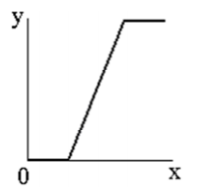
\includegraphics[width=0.22\textwidth]{images/funcLinStreach.png}
\caption{Функция линейного контрастирования изображения}
\label{fig:funcLinStreach}
\end{figure}

\begin{figure}[h!]
\centering
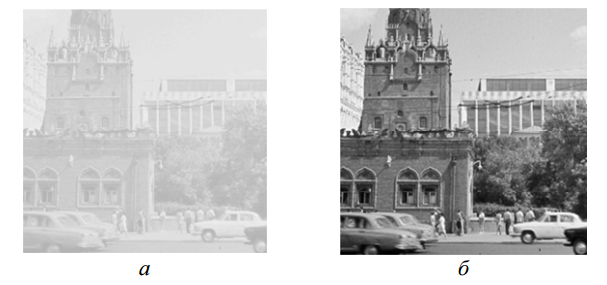
\includegraphics[width=0.8\textwidth]{images/linStreachExample.png}
\caption{ Пример линейного растяжения гистограммы}
\label{fig:exampleLinStreach}
\end{figure}
